\chapter{Le projet tuteuré}
Bien qu'il ait déjà fait l'objet d'un compte rendu détaillé de réalisation, je ne peux pas faire une synthèse de mon année sans mentionner mon projet tuteuré.

~

Bien évidemment, ce chapitre a pour but de donner seulement un aperçu de mon projet tuteuré. Si vous souhaitez en savoir plus à son propos, je vous conseille de vous référer au compte rendu détaillé qui lui est consacré. Attention, ce rapport est dit \og technique \fg, c'est-à-dire qu'il s'adresse à un public familier de l'informatique et du développement d'applications. Il est disponible ici : \url{https://github.com/downloads/darkelfe/Rapports/LicenceProfesionnelleDASI_ProjetTuteure_Rapport.pdf}.

\section{Présentation}
\subsection{Origine du module}
Parmi les nombreuses fonctionnalités proposées par \integrale, il existe plusieurs possibilités d'envoi automatique de documents. En effet, l'organisation du transport international nécessite l'envoi de divers documents officiels, par exemple à la douane, ou à la compagnie maritime pour réserver des emplacement sur un bateau, etc. A l'ère de l'informatique, tous ces documents sont désormais électroniques mais un problème majeur reste : il peuvent être très compliqués à rédiger.

C'est pour cette raison qu'\integrale{} propose d'écrire automatiquement ces documents, en y incluant toutes les informations nécessaires, et de les envoyer à son destinataire par un simple clic sur un bouton.

~

Dans le cadre du projet tuteuré, nous devons nous concentrer sur un seul de ces documents : le \emph{Boat Landing}, généralement abrégé en
\og BL \fg. Il s'agit d'un fichier émit à l'attention de la compagnie maritime qui détaille le contenu d'un projet : nombre et propriétés des conteneurs\footnote{Ici, il est fait référence aux conteneurs \emph{maritimes}, c'est-à-dire de \og grandes boites rectangulaires métalliques \fg.}, poids et volume des marchandises qui sont dedans, etc.

Une des particularités de ce fichier, c'est sa totale illisibilité par un être humain. Les informations qu'il contient doivent respecter une norme particulière qui ne facilite pas la lecture.

~

Pour simplifier le travail de nos clients, \solulog{} a donc décidé de créer un module qui écrit automatiquement ce fichier puis l'envoie par internet.

\subsection{\pireus}
Tout commence donc en 2006 avec Alexandre, qui est chargé de ce travail. Puisque \solulog{} souhaite pouvoir vendre ce futur module indépendamment de \integrale, il est décidé que le module, nommé \emph{\pireus}, sera écrit en PHP, avec seulement une petite partie en \vb{} pour transmettre les données nécessaires à la création du fichier.

~

Quelques temps plus tard, le module est prêt et mis en service. Les années passent et en 2009, Alexandre, le responsable du module et seul développeur, quitte \solulog. \pireus{} fonctionnant parfaitement, les choses restent comme cela.

Mais à la fin de la même année, \solulog{} se trouve dans l'obligation de le modifier pour y intégrer de nouvelles fonctionnalités. Or, personne, au sein de \solulog, ne maîtrise le PHP. Finalement, c'est Samuel qui se charge des modifications. Malgré l'aide d'Alexandre, il a beaucoup de difficultés pour appréhender la totalité du module.

\subsection{Objectifs}
C'est cet événement qui va pousser \solulog{} à réfléchir au problème. Il va finalement en ressortir que le module doit être entièrement réécrit en \vb{} et intégré à \integrale, les tentatives de vente ayant été abandonnées.

~

Mon arrivée en 2010 leur donne l'occasion d'effectuer cette tâche. Je suis donc chargé, à titre de projet tuteuré, de réécrire entièrement le module PHP en \vb. Je dois également en profiter pour écrire une documentation complète sur mon module, afin de simplifier sa compréhension et les possibles modifications ultérieures.

\section{Déroulement du projet}
Mon projet tuteuré s'est déroulé en deux grandes parties, que je vais détailler ici.

\subsection{Phase 1 : rédaction du nouveau module}
La première partie, qui se déroule sur l'ensemble des mois d'octobre et de novembre 2010, a eu pour objectif principal la création du nouveau module.

~

Cette première phase est elle-même découpée en sept tâches successives.

\subsubsection{Analyse de l'existant}
Au tout début, avant même de penser à réécrire \pireus, il faut commencer par savoir de quoi traite ce module et comment il est construit. J'ai donc commencé par l'étudier et observer la manière dont est organisé son contenu (fichiers source, etc.). Ensuite, je me suis lancé dans l'étude du code PHP lui-même. J'ai eu beaucoup de mal, notamment en l'absence d'une documentation claire et de l'utilisation de fonctions que je ne connaissais pas encore. Mais j'ai quand même réussi à identifier la majorité des données fournies par l'utilisateur dans le fichier final.

\subsubsection{Récupération des valeurs}
Les valeurs fournies par l'utilisateur sont stockées dans la base de données. La première chose que j'ai donc dû faire dans mon nouveau module, nommé \emph{BL\_INTTRA}, a été de lire ces valeurs et de les placer en mémoire, afin qu'elles soient facilement accessibles par la suite. J'ai eu quelques désaccords avec mon supérieur sur la manière de stocker les valeurs en question, mais nous sommes finalement parvenus à un compromis.

\subsubsection{Tests des valeurs}
Les valeurs fournies par l'utilisateur peuvent contenir des erreurs, des éléments incompatibles avec les BL, et il peut également manquer des informations essentielles. Donc, avant de générer le fichier de BL final, j'ai dû tester toutes les valeurs lues. Heureusement pour moi, ces tests étaient déjà présents dans le module d'Alexandre. J'ai donc seulement eu à les convertir en \vb{} et les intégrer à mon module. J'ai tout de même réorganisé l'ordre des tests pour que ceux-ci soient groupés en fonction du type des données sur lesquelles ils portaient.

\subsubsection{Génération du BL}
A ce moment-là, tout est prêt pour générer le message de BL. Avec l'aide de \pireus{} et de la documentation officielle de la norme \emph{IFTMIN D99B}\footnote{Il s'agit d'une norme régissant le contenu des fichiers de BL.}, j'ai entrepris la longue et difficile tâche de générer le BL. Cette partie n'a pas été sans mal. J'ai eu de nombreux problèmes, notamment pour calculer certaines variables essentielles au fichier final (poids des marchandises, numéro de révision, etc.), mais j'ai finalement réussi à m'en sortir.

\subsubsection{Écriture d'une documentation}
Comme c'était initialement prévu, j'ai dû écrire une documentation portant sur la génération d'un BL. J'ai profité du fait que les segments\footnote{Un segment est un fragment d'un fichier de BL. Il sont séparés par des apostrophes : \og ' \fg.} et leurs particularités étaient encore frais dans mémoire pour réaliser celle-ci. Une première partie de la documentation détaille l'ensemble des tests à mener sur les valeurs avant d'écrire le BL. Je détaille donc les conditions des tests, plusieurs n'étant obligatoire que dans certains cas précis. La valeur à tester ainsi que les possibles tests qui peuvent en découler peuvent dépendre d'une valeur particulière, comme le Brésil pour le port de destination.

La seconde partie de la documentation porte sur les segments : liste et ordre d'apparition dans le BL, mais également lesquels sont obligatoires, les valeurs qu'ils contiennent ou encore si ces valeurs sont elles-mêmes obligatoires.

~

Voici deux exemples de segments issus de ma documentation :
\begin{figure}[h!]
	\begin{center}
		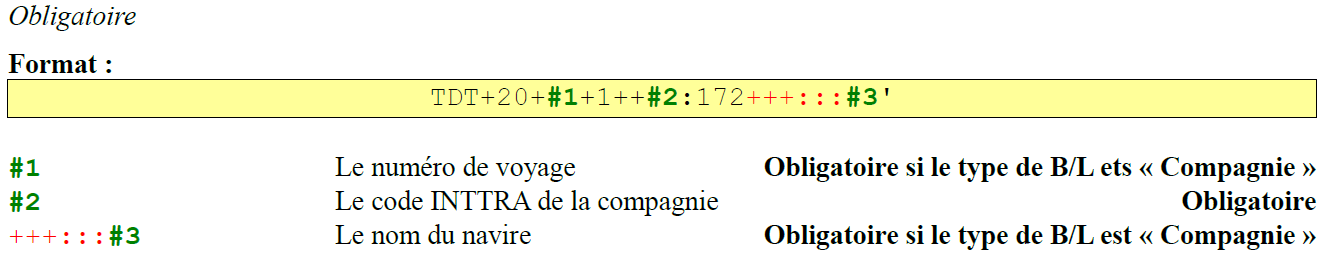
\includegraphics[scale=.54]{Contenu/Synthese_SeptembreAvril/Images/Segment_TDT.png}
	\end{center}

	\caption{Détail du segment \og TDT \fg}
	\label{segment_TDT}
\end{figure}
\begin{figure}[h!]
	\begin{center}
		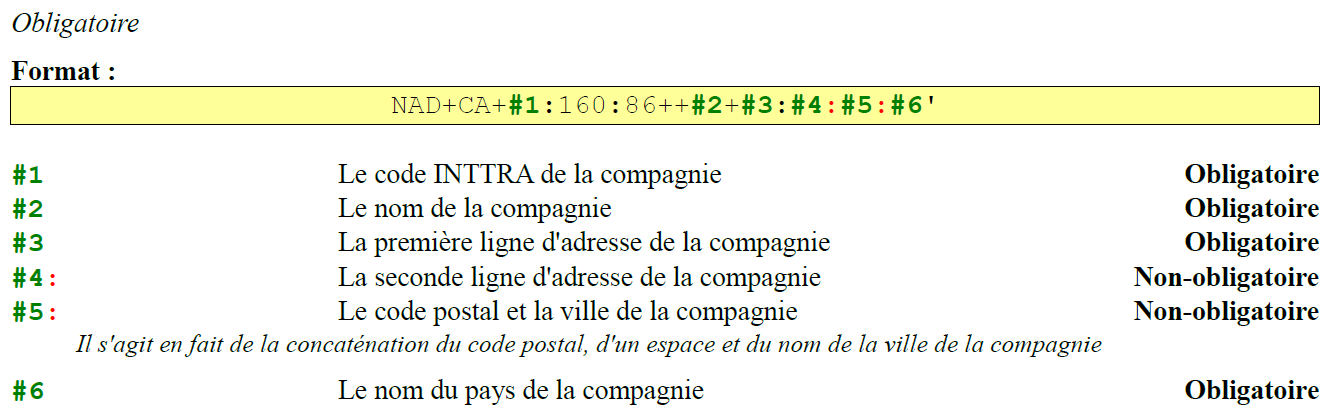
\includegraphics[scale=.54]{Contenu/Synthese_SeptembreAvril/Images/Segment_NAD_CA.png}
	\end{center}

	\caption{Détail du segment \og NAD-CA \fg}
	\label{segment_NAD_CA}
\end{figure}

\subsubsection{Test du module}
Une fois la génération des BL fonctionnelle, il a fallu la tester. Il y a trois types de tests différents successifs. Le premier test a consisté à vérifier le fichier obtenu par un outil de test fourni par la norme : \og EDI Test Tool Kit \fg.

Ensuite, avec de fausses données entrées manuellement, j'ai comparé mes résultats avec ceux de \pireus, portant bien sûr sur les mêmes données. Cela m'a permis de corriger plusieurs oublis de ma part.

Pour finir, mon module a été installé sur le serveur de test d'un de nos client. A partir de cela, j'ai pu faire fonctionner \emph{BL\_INTTRA} sur de véritables données. J'ai également pu tester les résultats en les comparant aux fichiers générés chez le client.

\subsubsection{Envoi par FTP}
Il s'agit de la partie la plus simple et la plus courte de mon projet tuteuré : envoyer le BL généré à l'organisme correspondant par internet, par le biais du protocole FTP. Par chance, Alexandre avait déjà réalisé par le passé un ensemble de fonctions simplifiant à l'extrême l'envoi et la récupération de fichiers par FTP. J'ai donc simplement réutilisé ces fonctions pour faire mon envoi.

\subsection{Phase 2 : Intégration et évolution}
La seconde partie de mon projet tuteuré s'est déroulée plus tard dans l'année, à la jonction entre le mois de décembre 2010 et celui de janvier 2011. Ma principale mission était d'intégrer définitivement mon module à \integrale{} et d'y ajouter quelques fonctionnalités.

\subsubsection{Récupération des statuts}
Lorsqu'un client envoie un BL, la société réceptrice met à sa disposition un autre document permettant de connaître l'état du BL : en cours de traitement, validé ou refusé. \pireus{} se chargeant déjà d'aller récupérer ces statuts par le passé, j'ai été amené à le faire. Au final, le traitement est très simple : aller récupérer les statuts par FTP, puis les analyser. J'ai profité de cette réécriture pour simplifier le processus du module d'Alexandre. En effet, celui-ci extrayait beaucoup d'informations inutiles du message de statut. Dans mon module, je me contente de récupérer le statut lui-même et d'en avertir l'utilisateur de celui-ci.

\subsubsection{Intégration}
Dans un premier temps, j'ai terminé de placer mon module dans \integrale. À ce moment là, mon module était déjà physiquement présent dans le logiciel. De même, appuyer sur le bouton de génération provoquait un appel à mon module. Mais étant donné que \emph{BL\_INTTRA} était tout neuf, \solulog{} n'a souhaité l'intégrer qu'à la seule condition qu'il y ait une solution de repli : si mon module échoue à générer un BL, il fallait que le client puisse facilement utiliser \pireus. J'ai donc choisi mettre en place un petit système de choix. Chaque utilisateur, dans son paramétrage, peut décider d'utiliser mon module ou celui d'Alexandre. Ensuite, lorsqu'il clique sur le bouton de génération d'un BL, \integrale{} appelle le système correspondant.

\subsubsection{Recette}
Bien que cette étape ait été prévue pour plus tard dans l'année (aux alentours du mois d'avril), la mise en place du module chez le client s'est produite bien plus tôt que prévus suite à un appel d'un client. En effet, ce dernier avait tenté de générer un BL contenant trente-quatre conteneurs. Le problème est que la norme impose un maximum de trente marchandises par conteneur, et cent conteneurs maximum par BL. Cependant \pireus{} avait un défaut de conception qui avait pour conséquence d'inverser ces deux limites. Donc impossible pour notre client de générer le BL. Face à l'urgence de la situation, \solulog{} a décidé de mettre en place mon module directement chez le client. C'est ainsi que la recette de mon module a démarré.

\subsubsection{Intégration des NVOCC}
Le dernier point de mon projet tuteuré était d'ajouter à mon module une fonctionnalité absente de \pireus{} : la gestion des \emph{NVOCC}. Les NVOCC sont des compagnies maritimes un peu particulières, qui n'ont pas exactement les mêmes exigences qu'une compagnie maritime standard. Par exemple, le numéro des conteneurs n'est plus obligatoire dans le cas d'une NVOCC. Cela influe sur les tests qui doivent être effectués lors de la génération d'un BL. Donc, \emph{via} la documentation officielle des BL à propos des NVOCC, j'ai modifié mes tests en fonction du type de compagnie maritime (standard ou NVOCC). J'ai également groupé d'un côté les fonctions propres aux NVOCC, et le reste d'un autre côté.
